\section{Технологический раздел}

В данном разделе определяются инструменты разработки средства распознавания суицидальных паттернов поведения человека по текстовым сообщениям.
Представлен интерфейс разработанного средства.

Приводится описание обрабатываемых данных, а также анализ тональности сообщений и облаков слов каждого класса.

\subsection{Выбор инструментов разработки}

Для организации хранения данных и моделей задействована реляционная СУБД PostgreSQL~\cite{postgres}. 
Данный выбор обусловлен наличием реляционных отношений в описанной системе, а также количеством полей у каждой сущности меньше 10, таким образом, данная СУБД может удовлетворить все потребности при реализации.

В качестве средства разработки метода распознавания суицидальных паттернов поведения человека по текстовым сообщениям использовался ЯП Python. Данный выбор обусловлен следующими факторами:

\begin{itemize}
	\item большое количество реализаций средств анализа и предобработки текста;
	\item широкий выбор библиотек для разработки в области машинного обучения;
	\item просто синтаксиса языка и высокая скорость разработки.
\end{itemize}

В качестве среды разработки был задействован Visual Studio Code. Данный выбор обусловлен тем, что это ПО распространяется по свободной лицензии, поставляется для конечного пользователя с открытым исходным кодом, а также имеет большое число расширений, ускоряющих процесс разработки.

Список задействованных в разработанном методе библиотек:
\begin{itemize}
	\item pandas~\cite{pandas} -- библиотека для обработки и анализа данных;
	\item numpy~\cite{numpy} -- библиотека, добавляющая поддержку больших многомерных массивов и матриц, вместе с большой библиотекой высокоуровневых математических функций для операций с этими массивами;
	\item matplotlib~\cite{matplotlib} -- библиотека для визуализации данных;
	\item scikit-learn~\cite{sklearn} -- библиотека множества операций и алгоритмов, используемых в сфере науки о данных и машинном обучении;
	\item nltk~\cite{nltk} -- библиотека, предоставляющая обширный набор инструментов для работы с естественными языками;
	\item pymorphy2~\cite{pymorphy} -- библиотека, предоставляющая морфологический анализатор, а также утилиты для взаимодействия с ним.
\end{itemize}

\subsection{Интерфейс средства распознавания суицидальных паттернов поведения человека по текстовым сообщениям}

На рисунках \ref{img:utility1} и \ref{img:utility2} представлен интерфейс реализованного средства распознавания суицидальных паттернов поведения человека по текстовым сообщениям. Средство позволяет выбрать пользователю как модель, так и метод векторизации сообщения, поступающего в систему.

\begin{figure}[H]
	\centering
	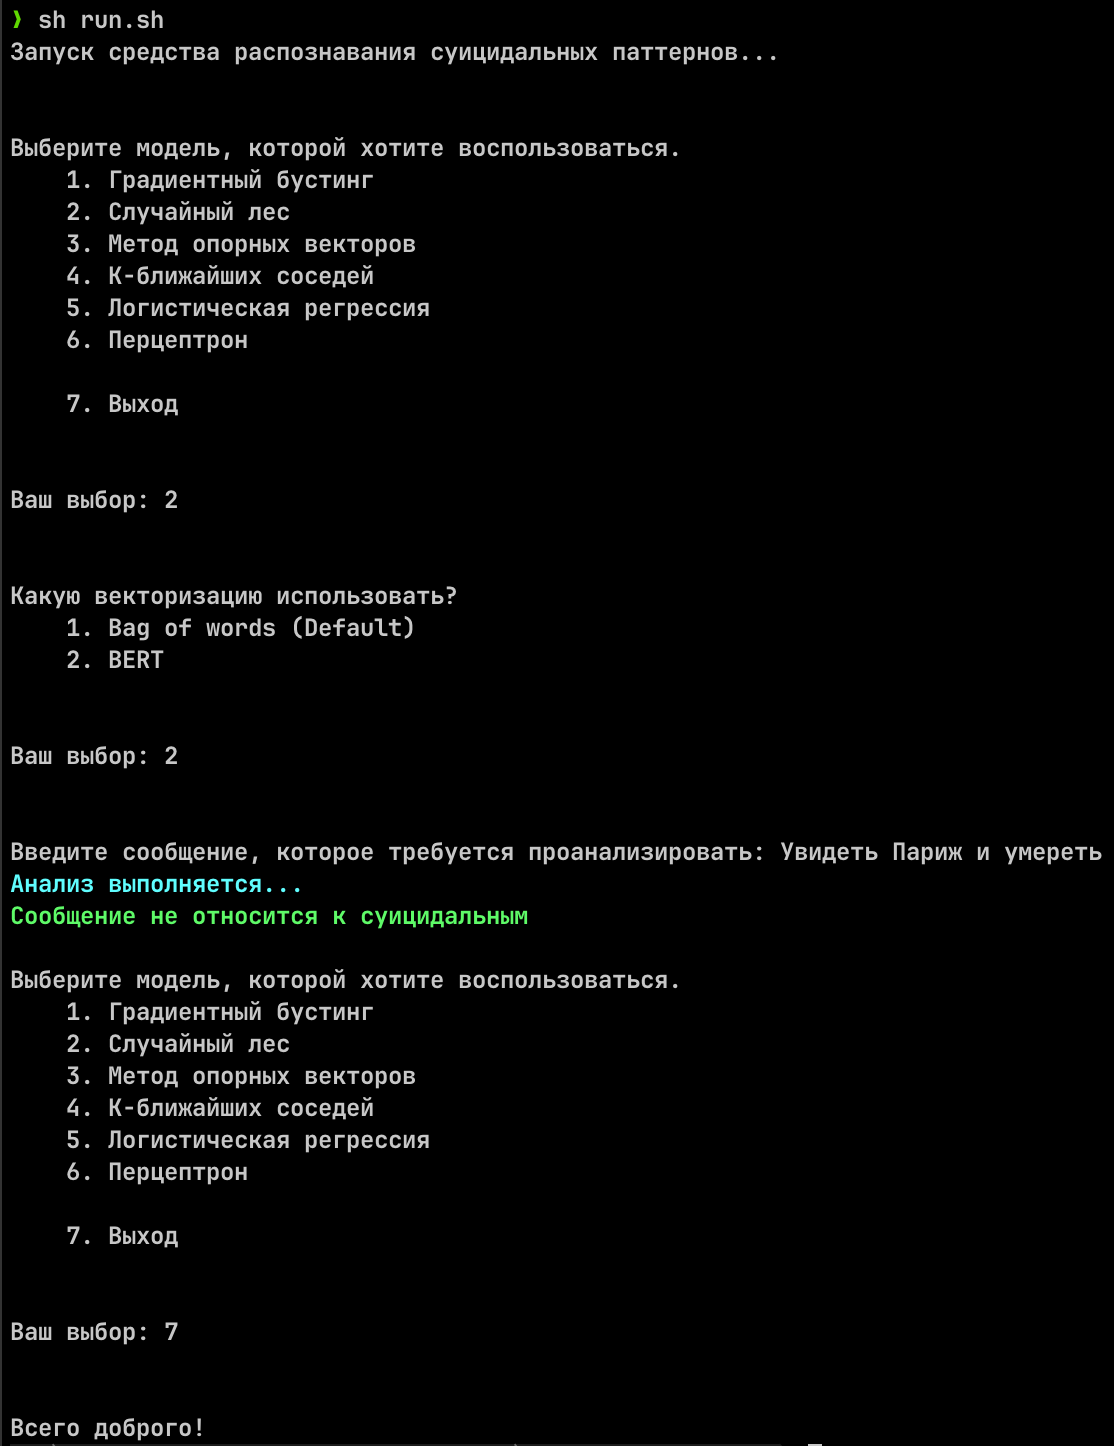
\includegraphics[width=\textwidth]{inc/utility1.png}
	\caption{ Полная пользовательская история использования средства. }
	\label{img:utility1}
\end{figure}

\begin{figure}[H]
	\centering
	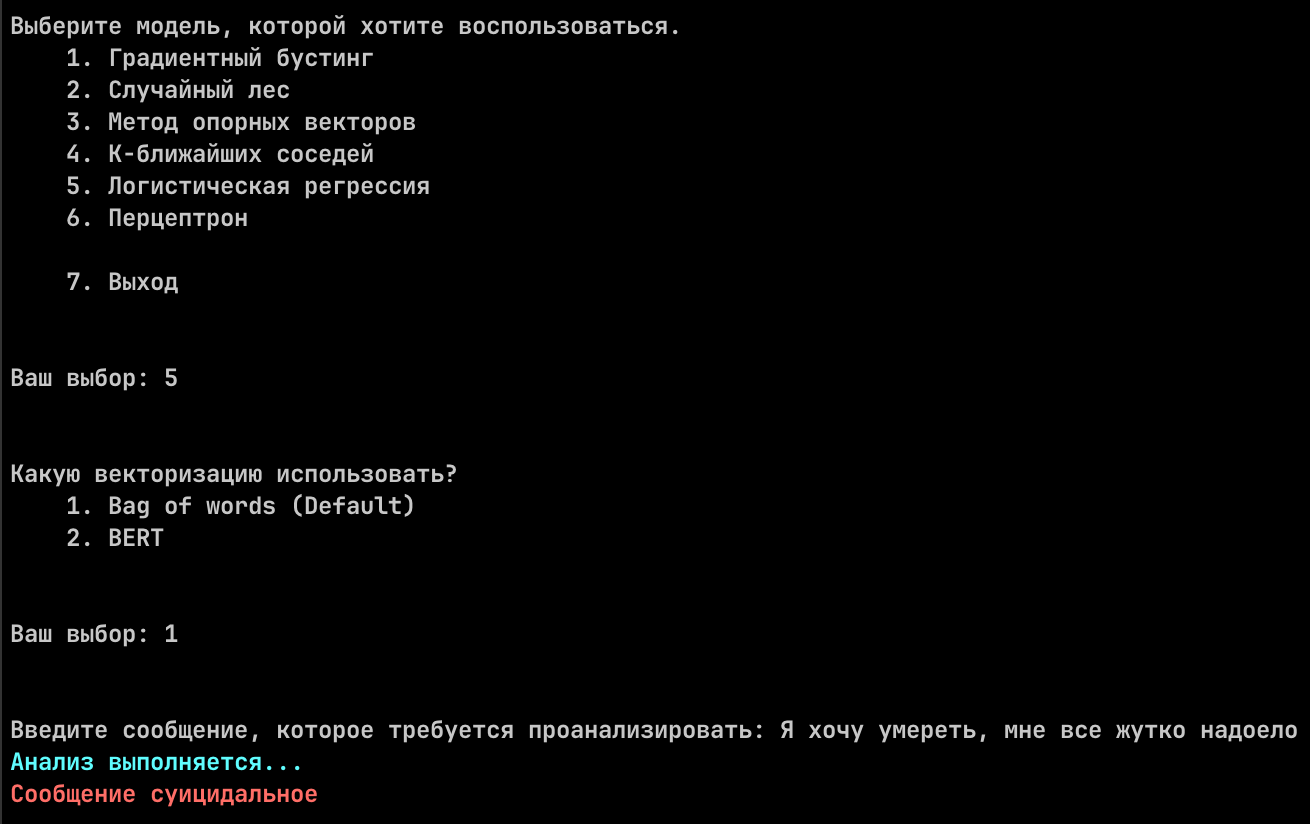
\includegraphics[width=\textwidth]{inc/utility2.png}
	\caption{ Результат анализа суицидального сообщения. }
	\label{img:utility2}
\end{figure}

\subsection{Описание обрабатываемых данных}

В результате работы средства сбора данных было размечено 1000 суицидальных сообщений. К собранным сообщениям было добавлено еще 1000 несуицидальных сообщений из датасета обнаружения пресуицидальных сигналов~\cite{dataset}. 

На рисунках \ref{img:sentiments1} и \ref{img:sentiments2} представлены круговые диаграммы тональности сообщений, полученные с использованием библиотеки Dostoevsky \cite{dostoevsky}.

\begin{figure}[H]
	\centering
	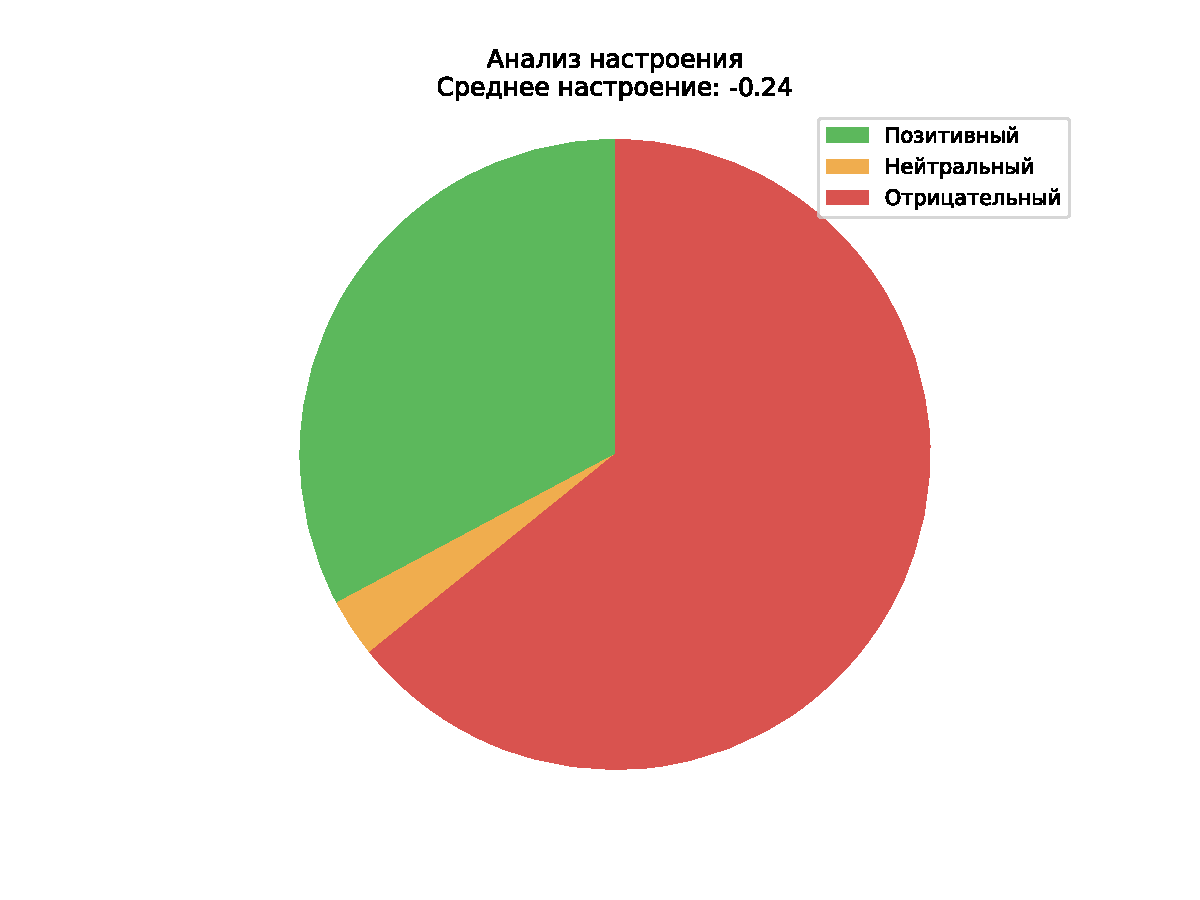
\includegraphics[width=0.8\textwidth]{inc/plots/sentiments_suicidal.pdf}
	\caption{ Круговая диаграмма тональности суицидальных сообщений. }
	\label{img:sentiments1}
\end{figure}

\begin{figure}[H]
	\centering
	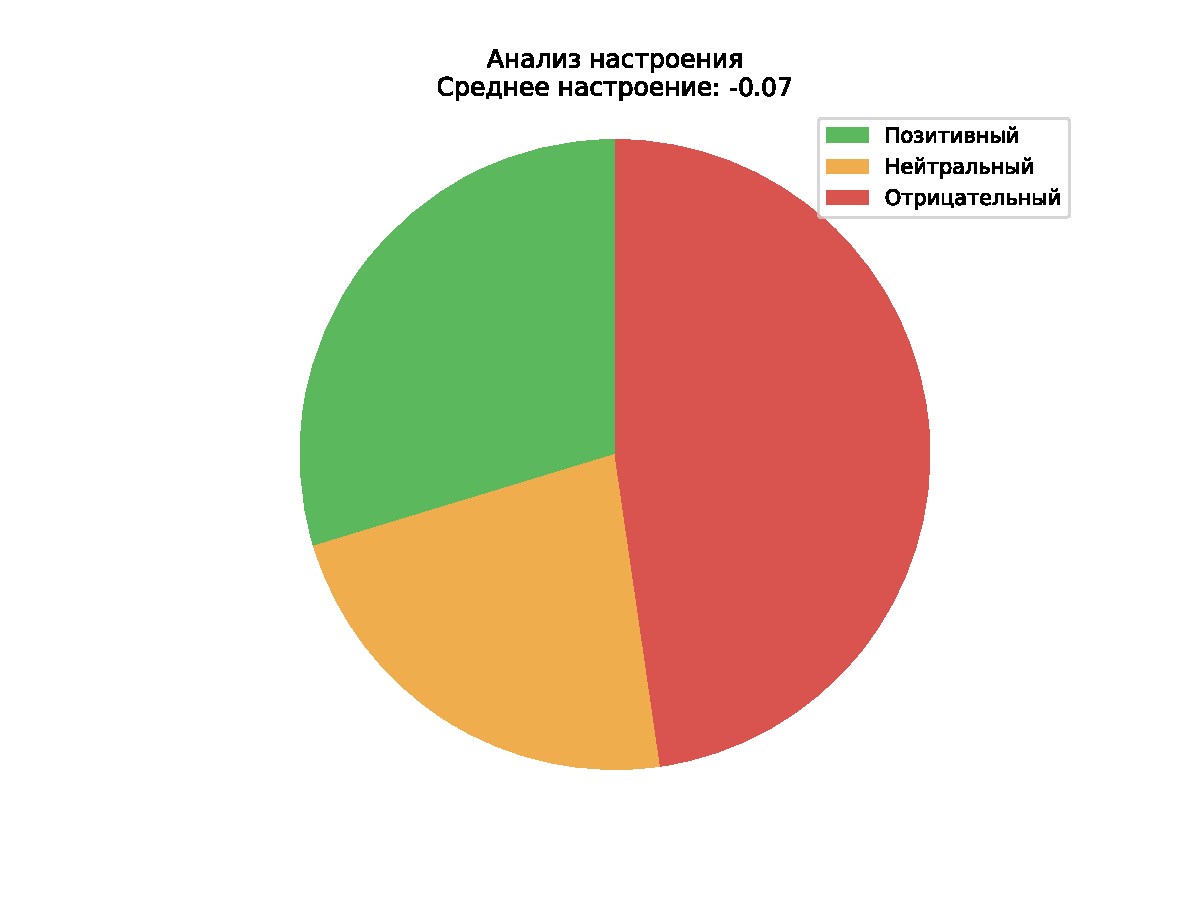
\includegraphics[width=0.8\textwidth]{inc/plots/sentiments_non_suicidal.pdf}
	\caption{ Круговая диаграмма тональности несуицидальных сообщений. }
	\label{img:sentiments2}
\end{figure}

Представленные диаграммы показывают, что практически треть суицидальных сообщений автоматизированное средство оценки тональности распознает как сообщения с отрицательной окраской. Однако наличие среди них позитивно настроенных сообщений -- ошибка распознавания модели. Среди несуицидальных сообщений преобладают тексты с отрицательной окраской, однако тут их уже меньше половины, а нейтральных сообщений почти что четверть из всех представленных. 

На рисунке \ref{img:cloud1} представлена визуализация собранных данных класса суицидальных сообщений. Чаще всего в суицидальных сообщениях фигурируют слова ``жизнь'' (585 раз), ``хотеть'' (556 раз), ``человек'' (491 раз) и ``мочь'' (452 раза). Также стоит обратить внимание на присутствие слов ``суицид'', ``страдать'', ``депрессия'', ``смерть'', ``умирать'' и ``ад''.

\begin{figure}[H]
	\centering
	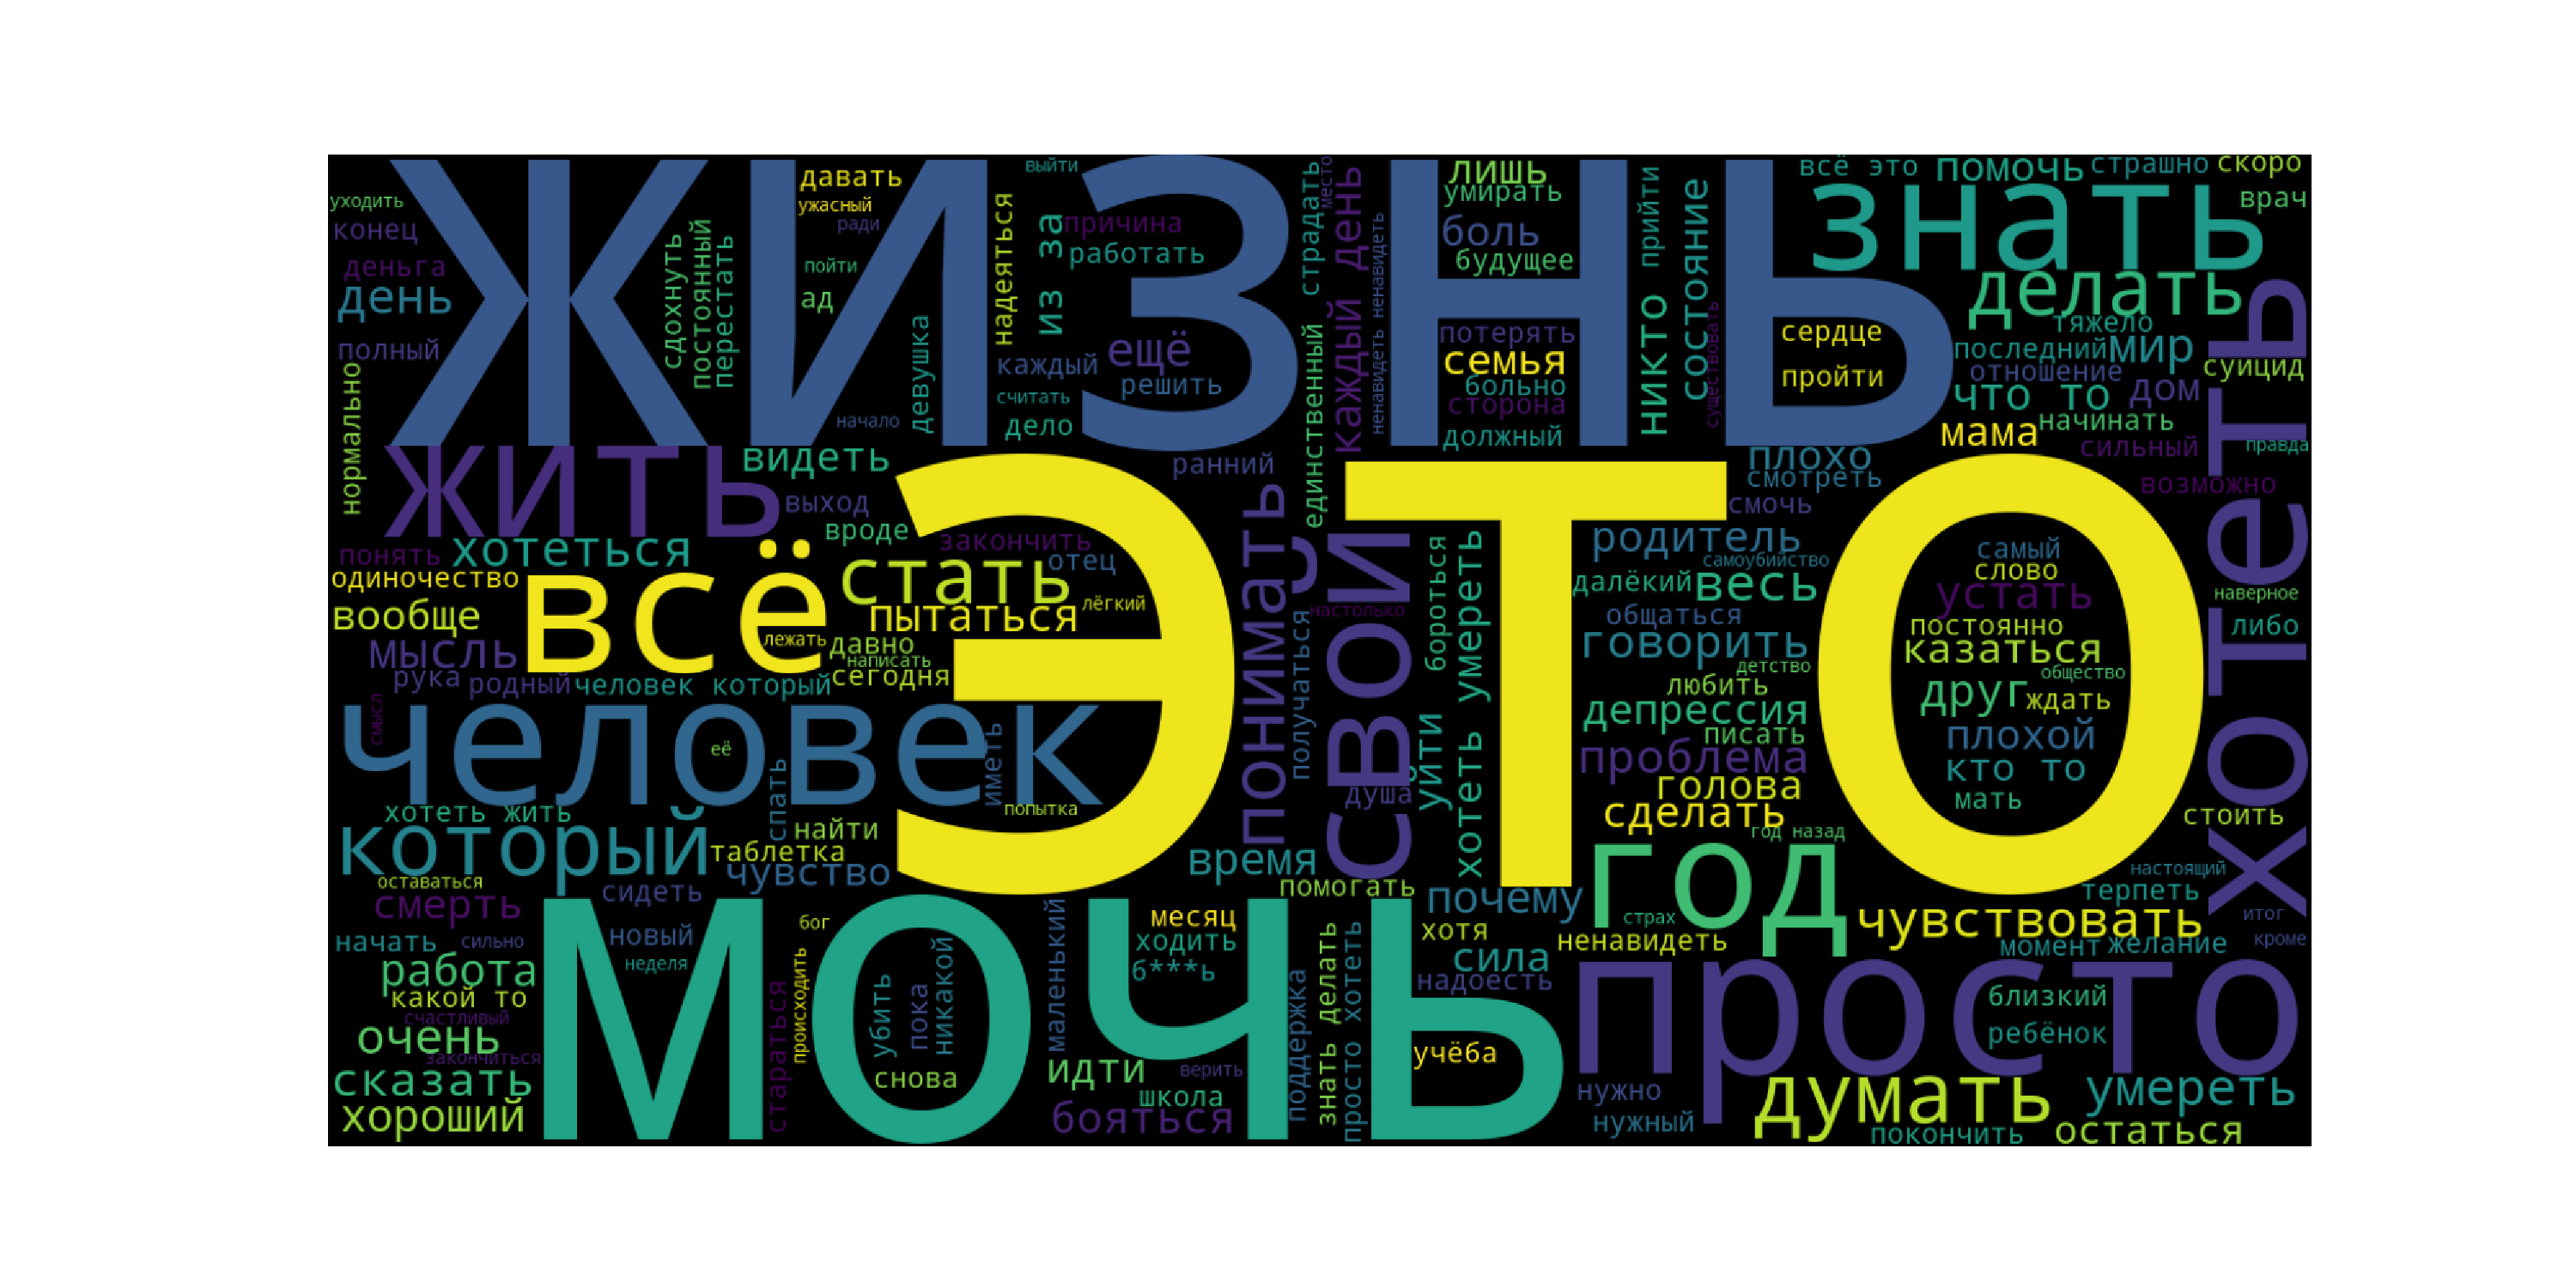
\includegraphics[width=\textwidth]{inc/cloudSuicidal.pdf}
	\caption{ Облако слов класса суицидальных сообщений. }
	\label{img:cloud1}
\end{figure}

На рисунке \ref{img:cloud2} представлена визуализация данных класса несуицидальных сообщений. Чаще всего в несуицидальных сообщениях встречаются слова ``хотеть'' (159 раз) и ``человек'' (67 раз). Кроме того сообщения данной тематики чаще включают в себя различные вариации нецензурной брани.

\begin{figure}[H]
	\centering
	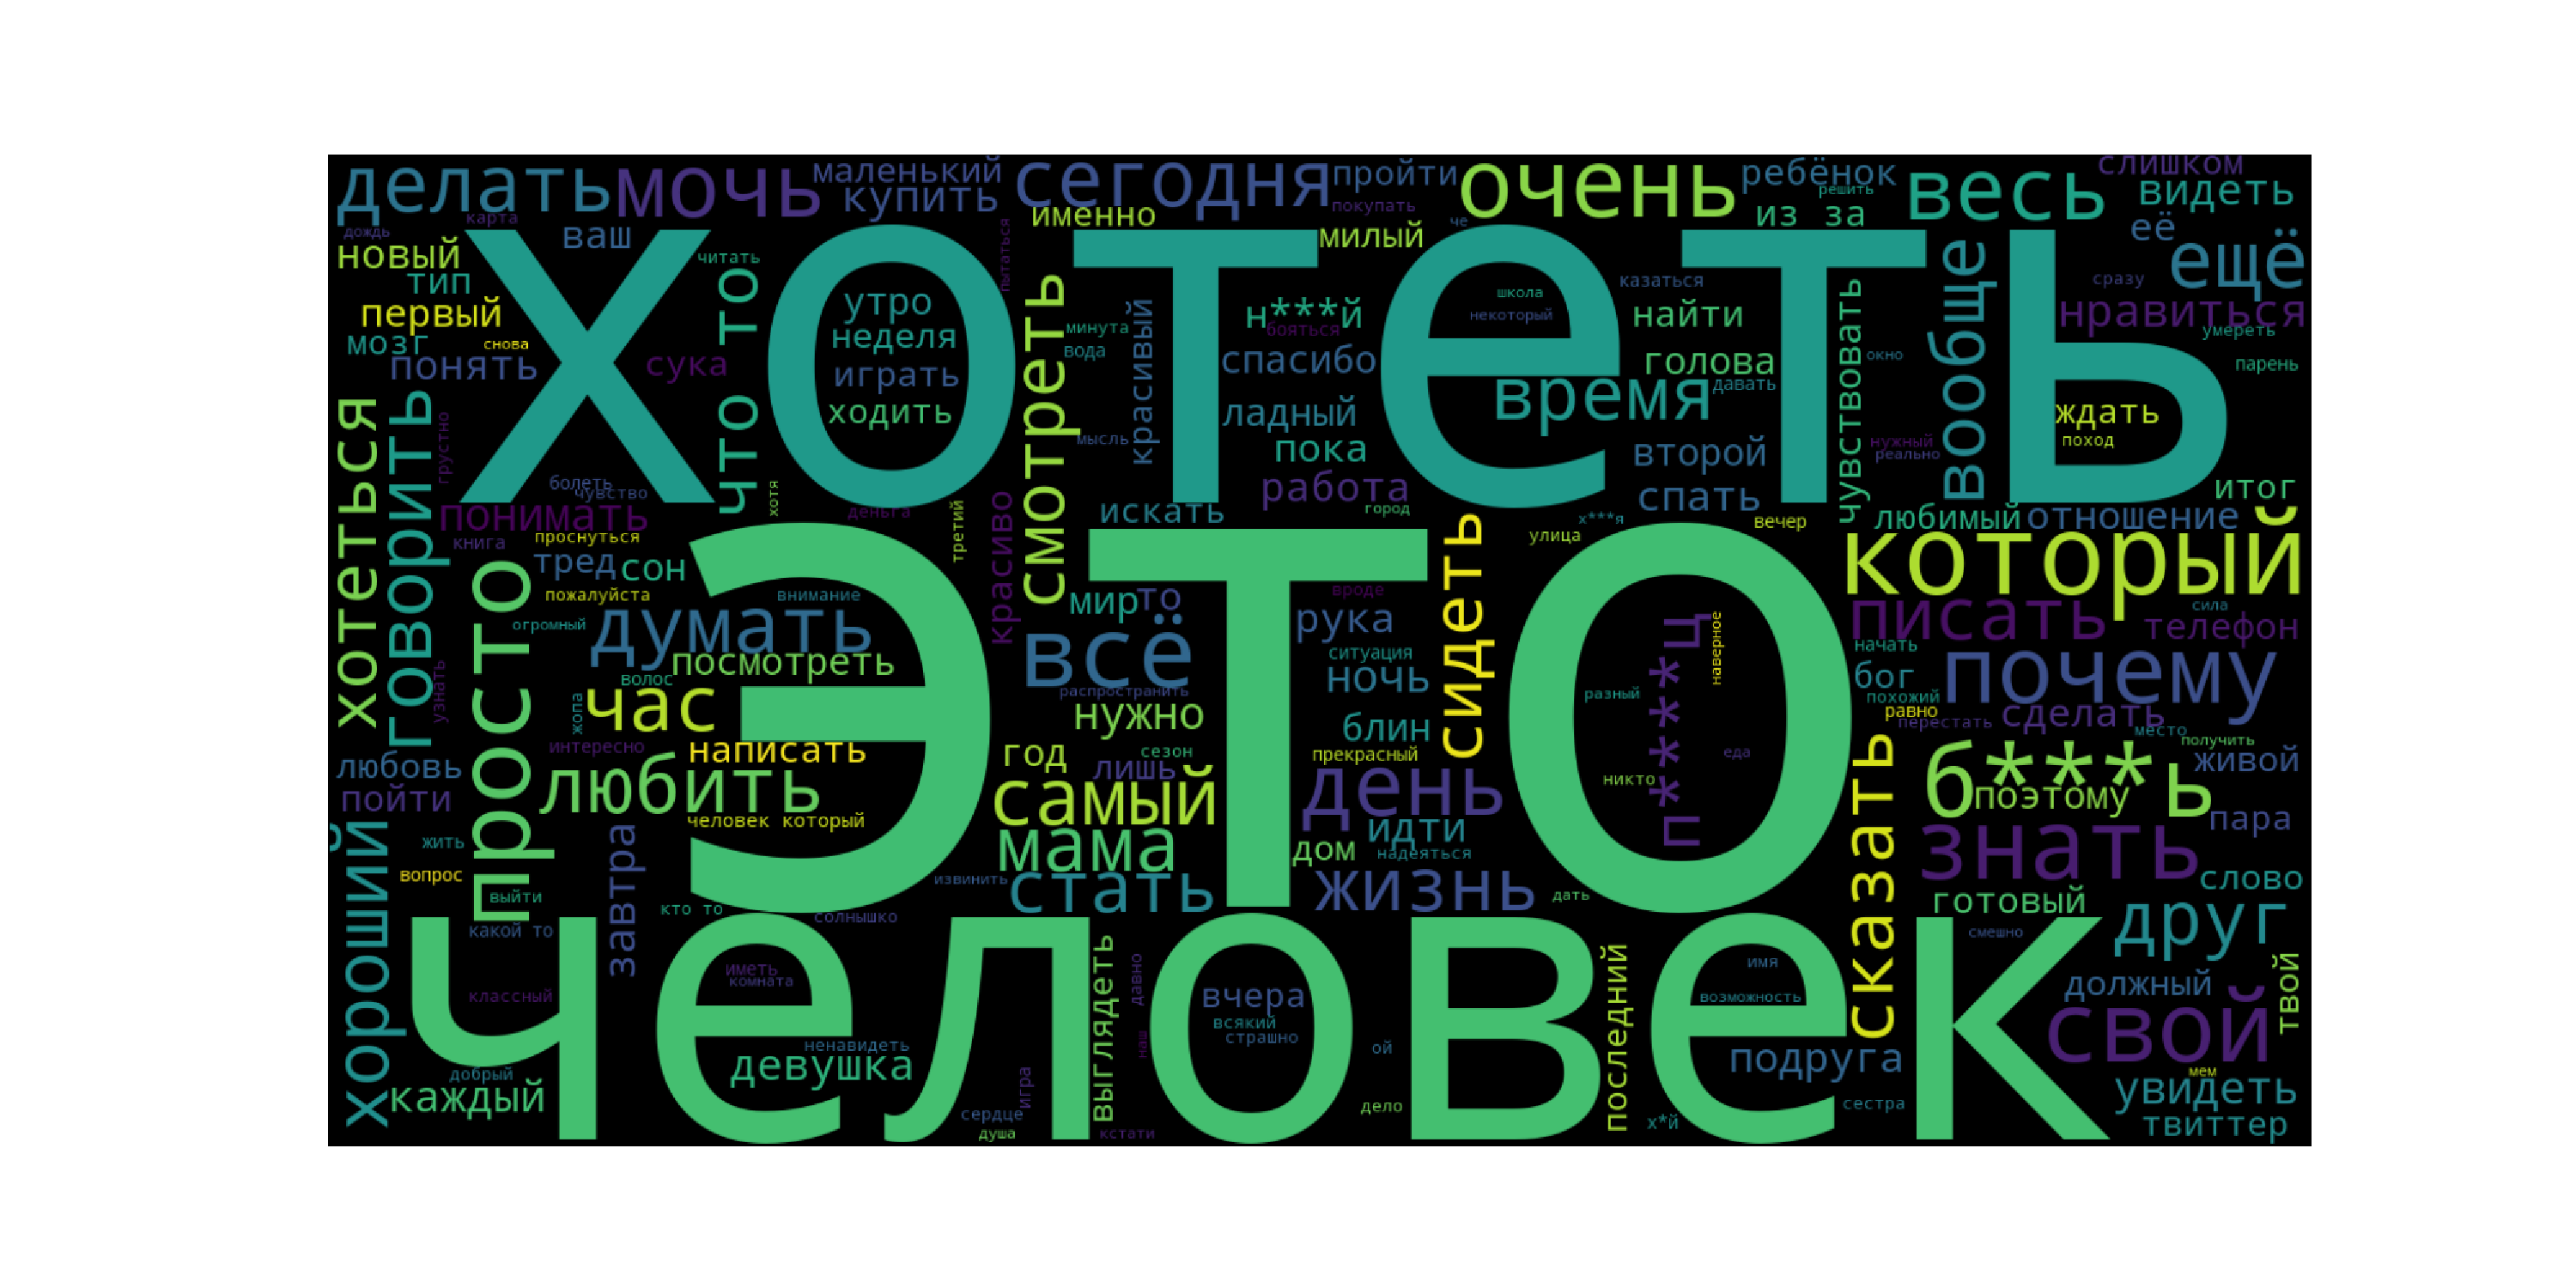
\includegraphics[width=\textwidth]{inc/cloudNonSuicidal.pdf}
	\caption{ Облако слов класса несуицидальных сообщений. }
	\label{img:cloud2}
\end{figure}

Представленная информация подтверждает факт того, что выбранные классы разделимы и отличны частотой употребления как слов, так и тематик. Кроме того, стоит отметить, что слово ``хотеть'' встречается в суицидальных сообщениях в $\approx 7.83$ раза чаще, чем в несуицидальных, а слово ``человек'' -- в $\approx 7.33$ раза чаще. Таким образом, суицидальные сообщения являются менее ``разнообразными'' и фиксирующимися на определенном словарном множестве.

\subsection*{Вывод}

В качестве языка разработки средства распознавания суицидальных паттернов поведения человека по текстовым сообщениям также будет использоваться ЯП Python. 
Задействованные библиотки: pandas, numpy, matplotlib, scikit-learn, nltk, pymorphy2.

Был представлен интерфейс средства распознавания суицидальных паттернов поведения человека по текстовым сообщениям.

Представленные диаграммы тональности сообщений показали, что практически треть суицидальных сообщений автоматизированное средство оценки тональности распознает как сообщения с отрицательной окраской. 
Среди несуицидальных сообщений преобладают тексты с отрицательной окраской, при этом нейтральных сообщений -- четверть из всех.

Визуализированные облака слов подтвердили гипотезу, что выбранные классы суицидальных и несуицидальных сообщений разделимы и отличны частотой некоторых слов. 
Отмечено, что слово ``хотеть'' встречается в суицидальных сообщениях в $\approx 7.83$ раза чаще, чем в несуицидальных, а слово ``человек'' -- в $\approx 7.33$ раза чаще. 
Таким образом, суицидальные сообщения являются менее ``разнообразными'' и фиксирующимися на определенном словарном множестве.
